% Options for packages loaded elsewhere
\PassOptionsToPackage{unicode}{hyperref}
\PassOptionsToPackage{hyphens}{url}
%
\documentclass[
]{article}
\usepackage{amsmath,amssymb}
\usepackage{iftex}
\ifPDFTeX
  \usepackage[T1]{fontenc}
  \usepackage[utf8]{inputenc}
  \usepackage{textcomp} % provide euro and other symbols
\else % if luatex or xetex
  \usepackage{unicode-math} % this also loads fontspec
  \defaultfontfeatures{Scale=MatchLowercase}
  \defaultfontfeatures[\rmfamily]{Ligatures=TeX,Scale=1}
\fi
\usepackage{lmodern}
\ifPDFTeX\else
  % xetex/luatex font selection
\fi
% Use upquote if available, for straight quotes in verbatim environments
\IfFileExists{upquote.sty}{\usepackage{upquote}}{}
\IfFileExists{microtype.sty}{% use microtype if available
  \usepackage[]{microtype}
  \UseMicrotypeSet[protrusion]{basicmath} % disable protrusion for tt fonts
}{}
\makeatletter
\@ifundefined{KOMAClassName}{% if non-KOMA class
  \IfFileExists{parskip.sty}{%
    \usepackage{parskip}
  }{% else
    \setlength{\parindent}{0pt}
    \setlength{\parskip}{6pt plus 2pt minus 1pt}}
}{% if KOMA class
  \KOMAoptions{parskip=half}}
\makeatother
\usepackage{xcolor}
\usepackage[margin=1in]{geometry}
\usepackage{color}
\usepackage{fancyvrb}
\newcommand{\VerbBar}{|}
\newcommand{\VERB}{\Verb[commandchars=\\\{\}]}
\DefineVerbatimEnvironment{Highlighting}{Verbatim}{commandchars=\\\{\}}
% Add ',fontsize=\small' for more characters per line
\usepackage{framed}
\definecolor{shadecolor}{RGB}{248,248,248}
\newenvironment{Shaded}{\begin{snugshade}}{\end{snugshade}}
\newcommand{\AlertTok}[1]{\textcolor[rgb]{0.94,0.16,0.16}{#1}}
\newcommand{\AnnotationTok}[1]{\textcolor[rgb]{0.56,0.35,0.01}{\textbf{\textit{#1}}}}
\newcommand{\AttributeTok}[1]{\textcolor[rgb]{0.13,0.29,0.53}{#1}}
\newcommand{\BaseNTok}[1]{\textcolor[rgb]{0.00,0.00,0.81}{#1}}
\newcommand{\BuiltInTok}[1]{#1}
\newcommand{\CharTok}[1]{\textcolor[rgb]{0.31,0.60,0.02}{#1}}
\newcommand{\CommentTok}[1]{\textcolor[rgb]{0.56,0.35,0.01}{\textit{#1}}}
\newcommand{\CommentVarTok}[1]{\textcolor[rgb]{0.56,0.35,0.01}{\textbf{\textit{#1}}}}
\newcommand{\ConstantTok}[1]{\textcolor[rgb]{0.56,0.35,0.01}{#1}}
\newcommand{\ControlFlowTok}[1]{\textcolor[rgb]{0.13,0.29,0.53}{\textbf{#1}}}
\newcommand{\DataTypeTok}[1]{\textcolor[rgb]{0.13,0.29,0.53}{#1}}
\newcommand{\DecValTok}[1]{\textcolor[rgb]{0.00,0.00,0.81}{#1}}
\newcommand{\DocumentationTok}[1]{\textcolor[rgb]{0.56,0.35,0.01}{\textbf{\textit{#1}}}}
\newcommand{\ErrorTok}[1]{\textcolor[rgb]{0.64,0.00,0.00}{\textbf{#1}}}
\newcommand{\ExtensionTok}[1]{#1}
\newcommand{\FloatTok}[1]{\textcolor[rgb]{0.00,0.00,0.81}{#1}}
\newcommand{\FunctionTok}[1]{\textcolor[rgb]{0.13,0.29,0.53}{\textbf{#1}}}
\newcommand{\ImportTok}[1]{#1}
\newcommand{\InformationTok}[1]{\textcolor[rgb]{0.56,0.35,0.01}{\textbf{\textit{#1}}}}
\newcommand{\KeywordTok}[1]{\textcolor[rgb]{0.13,0.29,0.53}{\textbf{#1}}}
\newcommand{\NormalTok}[1]{#1}
\newcommand{\OperatorTok}[1]{\textcolor[rgb]{0.81,0.36,0.00}{\textbf{#1}}}
\newcommand{\OtherTok}[1]{\textcolor[rgb]{0.56,0.35,0.01}{#1}}
\newcommand{\PreprocessorTok}[1]{\textcolor[rgb]{0.56,0.35,0.01}{\textit{#1}}}
\newcommand{\RegionMarkerTok}[1]{#1}
\newcommand{\SpecialCharTok}[1]{\textcolor[rgb]{0.81,0.36,0.00}{\textbf{#1}}}
\newcommand{\SpecialStringTok}[1]{\textcolor[rgb]{0.31,0.60,0.02}{#1}}
\newcommand{\StringTok}[1]{\textcolor[rgb]{0.31,0.60,0.02}{#1}}
\newcommand{\VariableTok}[1]{\textcolor[rgb]{0.00,0.00,0.00}{#1}}
\newcommand{\VerbatimStringTok}[1]{\textcolor[rgb]{0.31,0.60,0.02}{#1}}
\newcommand{\WarningTok}[1]{\textcolor[rgb]{0.56,0.35,0.01}{\textbf{\textit{#1}}}}
\usepackage{graphicx}
\makeatletter
\def\maxwidth{\ifdim\Gin@nat@width>\linewidth\linewidth\else\Gin@nat@width\fi}
\def\maxheight{\ifdim\Gin@nat@height>\textheight\textheight\else\Gin@nat@height\fi}
\makeatother
% Scale images if necessary, so that they will not overflow the page
% margins by default, and it is still possible to overwrite the defaults
% using explicit options in \includegraphics[width, height, ...]{}
\setkeys{Gin}{width=\maxwidth,height=\maxheight,keepaspectratio}
% Set default figure placement to htbp
\makeatletter
\def\fps@figure{htbp}
\makeatother
\setlength{\emergencystretch}{3em} % prevent overfull lines
\providecommand{\tightlist}{%
  \setlength{\itemsep}{0pt}\setlength{\parskip}{0pt}}
\setcounter{secnumdepth}{-\maxdimen} % remove section numbering
\ifLuaTeX
  \usepackage{selnolig}  % disable illegal ligatures
\fi
\IfFileExists{bookmark.sty}{\usepackage{bookmark}}{\usepackage{hyperref}}
\IfFileExists{xurl.sty}{\usepackage{xurl}}{} % add URL line breaks if available
\urlstyle{same}
\hypersetup{
  pdftitle={Predictive Modeling Assignment 2},
  pdfauthor={Jordan Dever},
  hidelinks,
  pdfcreator={LaTeX via pandoc}}

\title{Predictive Modeling Assignment 2}
\author{Jordan Dever}
\date{2024-02-22}

\begin{document}
\maketitle

\hypertarget{carefully-explain-the-differences-between-the-knn-classifier-and-knn-regression-methods.}{%
\subsection{2. Carefully explain the differences between the KNN
classifier and KNN regression
methods.}\label{carefully-explain-the-differences-between-the-knn-classifier-and-knn-regression-methods.}}

One difference between KNN classifier and KNN regression is that in KNN
classifier, is that KNN regression would be used in situations where our
target variable is numeric / continuous where y is any number and we
would use KNN classifier if our target is categorical / discrete because
our y output is 0 or 1. KNN regression takes K and the prediction point
to find the nearest training points near the prediction point, then
tries to predict using the average of the nearest neighbors. KNN
classifier takes the points near the prediction point in the training
data and estimates the conditional probability of the class. KNN
classifier will then classify a test point to whichever class it had the
highest probability for.

\hypertarget{this-question-involves-the-use-of-multiple-linear-regression-on-the-auto-data-set.}{%
\subsection{9. This question involves the use of multiple linear
regression on the Auto data
set.}\label{this-question-involves-the-use-of-multiple-linear-regression-on-the-auto-data-set.}}

\begin{Shaded}
\begin{Highlighting}[]
\NormalTok{auto }\OtherTok{\textless{}{-}} \FunctionTok{read.csv}\NormalTok{(}\StringTok{"\textasciitilde{}/R{-}Studio/Predictive Modeling/ALL CSV FILES {-} 2nd Edition/Auto.csv"}\NormalTok{)}
\end{Highlighting}
\end{Shaded}

\begin{enumerate}
\def\labelenumi{(\alph{enumi})}
\tightlist
\item
  Produce a scatterplot matrix which includes all of the variables in
  the data set.
\end{enumerate}

\begin{Shaded}
\begin{Highlighting}[]
\FunctionTok{plot}\NormalTok{(auto)}
\end{Highlighting}
\end{Shaded}

\includegraphics{Predictive-Modeling-Assignment-2_files/figure-latex/unnamed-chunk-2-1.pdf}

\begin{enumerate}
\def\labelenumi{(\alph{enumi})}
\setcounter{enumi}{1}
\tightlist
\item
  Compute the matrix of correlations between the variables using the
  function cor(). You will need to exclude the name variable, cor()
  which is qualitative.
\end{enumerate}

\begin{Shaded}
\begin{Highlighting}[]
\NormalTok{auto\_no\_name }\OtherTok{=}\NormalTok{ auto }\SpecialCharTok{\%\textgreater{}\%} 
\NormalTok{  dplyr}\SpecialCharTok{::}\FunctionTok{select}\NormalTok{(}\SpecialCharTok{{-}}\NormalTok{name)}
\NormalTok{auto\_no\_name}\SpecialCharTok{$}\NormalTok{horsepower }\OtherTok{=} \FunctionTok{as.numeric}\NormalTok{(auto\_no\_name}\SpecialCharTok{$}\NormalTok{horsepower)}
\end{Highlighting}
\end{Shaded}

\begin{verbatim}
## Warning: NAs introduced by coercion
\end{verbatim}

\begin{Shaded}
\begin{Highlighting}[]
\FunctionTok{cor}\NormalTok{(auto\_no\_name)}
\end{Highlighting}
\end{Shaded}

\begin{verbatim}
##                     mpg  cylinders displacement horsepower     weight
## mpg           1.0000000 -0.7762599   -0.8044430         NA -0.8317389
## cylinders    -0.7762599  1.0000000    0.9509199         NA  0.8970169
## displacement -0.8044430  0.9509199    1.0000000         NA  0.9331044
## horsepower           NA         NA           NA          1         NA
## weight       -0.8317389  0.8970169    0.9331044         NA  1.0000000
## acceleration  0.4222974 -0.5040606   -0.5441618         NA -0.4195023
## year          0.5814695 -0.3467172   -0.3698041         NA -0.3079004
## origin        0.5636979 -0.5649716   -0.6106643         NA -0.5812652
##              acceleration       year     origin
## mpg             0.4222974  0.5814695  0.5636979
## cylinders      -0.5040606 -0.3467172 -0.5649716
## displacement   -0.5441618 -0.3698041 -0.6106643
## horsepower             NA         NA         NA
## weight         -0.4195023 -0.3079004 -0.5812652
## acceleration    1.0000000  0.2829009  0.2100836
## year            0.2829009  1.0000000  0.1843141
## origin          0.2100836  0.1843141  1.0000000
\end{verbatim}

\begin{Shaded}
\begin{Highlighting}[]
\FunctionTok{is.na}\NormalTok{(auto\_no\_name}\SpecialCharTok{$}\NormalTok{horsepower)}
\end{Highlighting}
\end{Shaded}

\begin{verbatim}
##   [1] FALSE FALSE FALSE FALSE FALSE FALSE FALSE FALSE FALSE FALSE FALSE FALSE
##  [13] FALSE FALSE FALSE FALSE FALSE FALSE FALSE FALSE FALSE FALSE FALSE FALSE
##  [25] FALSE FALSE FALSE FALSE FALSE FALSE FALSE FALSE  TRUE FALSE FALSE FALSE
##  [37] FALSE FALSE FALSE FALSE FALSE FALSE FALSE FALSE FALSE FALSE FALSE FALSE
##  [49] FALSE FALSE FALSE FALSE FALSE FALSE FALSE FALSE FALSE FALSE FALSE FALSE
##  [61] FALSE FALSE FALSE FALSE FALSE FALSE FALSE FALSE FALSE FALSE FALSE FALSE
##  [73] FALSE FALSE FALSE FALSE FALSE FALSE FALSE FALSE FALSE FALSE FALSE FALSE
##  [85] FALSE FALSE FALSE FALSE FALSE FALSE FALSE FALSE FALSE FALSE FALSE FALSE
##  [97] FALSE FALSE FALSE FALSE FALSE FALSE FALSE FALSE FALSE FALSE FALSE FALSE
## [109] FALSE FALSE FALSE FALSE FALSE FALSE FALSE FALSE FALSE FALSE FALSE FALSE
## [121] FALSE FALSE FALSE FALSE FALSE FALSE  TRUE FALSE FALSE FALSE FALSE FALSE
## [133] FALSE FALSE FALSE FALSE FALSE FALSE FALSE FALSE FALSE FALSE FALSE FALSE
## [145] FALSE FALSE FALSE FALSE FALSE FALSE FALSE FALSE FALSE FALSE FALSE FALSE
## [157] FALSE FALSE FALSE FALSE FALSE FALSE FALSE FALSE FALSE FALSE FALSE FALSE
## [169] FALSE FALSE FALSE FALSE FALSE FALSE FALSE FALSE FALSE FALSE FALSE FALSE
## [181] FALSE FALSE FALSE FALSE FALSE FALSE FALSE FALSE FALSE FALSE FALSE FALSE
## [193] FALSE FALSE FALSE FALSE FALSE FALSE FALSE FALSE FALSE FALSE FALSE FALSE
## [205] FALSE FALSE FALSE FALSE FALSE FALSE FALSE FALSE FALSE FALSE FALSE FALSE
## [217] FALSE FALSE FALSE FALSE FALSE FALSE FALSE FALSE FALSE FALSE FALSE FALSE
## [229] FALSE FALSE FALSE FALSE FALSE FALSE FALSE FALSE FALSE FALSE FALSE FALSE
## [241] FALSE FALSE FALSE FALSE FALSE FALSE FALSE FALSE FALSE FALSE FALSE FALSE
## [253] FALSE FALSE FALSE FALSE FALSE FALSE FALSE FALSE FALSE FALSE FALSE FALSE
## [265] FALSE FALSE FALSE FALSE FALSE FALSE FALSE FALSE FALSE FALSE FALSE FALSE
## [277] FALSE FALSE FALSE FALSE FALSE FALSE FALSE FALSE FALSE FALSE FALSE FALSE
## [289] FALSE FALSE FALSE FALSE FALSE FALSE FALSE FALSE FALSE FALSE FALSE FALSE
## [301] FALSE FALSE FALSE FALSE FALSE FALSE FALSE FALSE FALSE FALSE FALSE FALSE
## [313] FALSE FALSE FALSE FALSE FALSE FALSE FALSE FALSE FALSE FALSE FALSE FALSE
## [325] FALSE FALSE FALSE FALSE FALSE FALSE  TRUE FALSE FALSE FALSE FALSE FALSE
## [337]  TRUE FALSE FALSE FALSE FALSE FALSE FALSE FALSE FALSE FALSE FALSE FALSE
## [349] FALSE FALSE FALSE FALSE FALSE FALSE  TRUE FALSE FALSE FALSE FALSE FALSE
## [361] FALSE FALSE FALSE FALSE FALSE FALSE FALSE FALSE FALSE FALSE FALSE FALSE
## [373] FALSE FALSE FALSE FALSE FALSE FALSE FALSE FALSE FALSE FALSE FALSE FALSE
## [385] FALSE FALSE FALSE FALSE FALSE FALSE FALSE FALSE FALSE FALSE FALSE FALSE
## [397] FALSE
\end{verbatim}

\begin{Shaded}
\begin{Highlighting}[]
\CommentTok{\#counted as ? in original data}
\end{Highlighting}
\end{Shaded}

\begin{enumerate}
\def\labelenumi{(\alph{enumi})}
\setcounter{enumi}{2}
\tightlist
\item
  Use the lm() function to perform a multiple linear regression with mpg
  as the response and all other variables except name as the predictors.
  Use the summary() function to print the results. Comment on the
  output. For instance: i. Is there a relationship between the
  predictors and the response? ii. Which predictors appear to have a
  statistically significant relationship to the response? iii. What does
  the coefficient for the year variable suggest?
\end{enumerate}

\begin{Shaded}
\begin{Highlighting}[]
\NormalTok{auto\_lm }\OtherTok{=} \FunctionTok{lm}\NormalTok{(mpg }\SpecialCharTok{\textasciitilde{}}\NormalTok{ ., }\AttributeTok{data =}\NormalTok{ auto\_no\_name)}
\FunctionTok{summary}\NormalTok{(auto\_lm)}
\end{Highlighting}
\end{Shaded}

\begin{verbatim}
## 
## Call:
## lm(formula = mpg ~ ., data = auto_no_name)
## 
## Residuals:
##     Min      1Q  Median      3Q     Max 
## -9.5903 -2.1565 -0.1169  1.8690 13.0604 
## 
## Coefficients:
##                Estimate Std. Error t value Pr(>|t|)    
## (Intercept)  -17.218435   4.644294  -3.707  0.00024 ***
## cylinders     -0.493376   0.323282  -1.526  0.12780    
## displacement   0.019896   0.007515   2.647  0.00844 ** 
## horsepower    -0.016951   0.013787  -1.230  0.21963    
## weight        -0.006474   0.000652  -9.929  < 2e-16 ***
## acceleration   0.080576   0.098845   0.815  0.41548    
## year           0.750773   0.050973  14.729  < 2e-16 ***
## origin         1.426141   0.278136   5.127 4.67e-07 ***
## ---
## Signif. codes:  0 '***' 0.001 '**' 0.01 '*' 0.05 '.' 0.1 ' ' 1
## 
## Residual standard error: 3.328 on 384 degrees of freedom
##   (5 observations deleted due to missingness)
## Multiple R-squared:  0.8215, Adjusted R-squared:  0.8182 
## F-statistic: 252.4 on 7 and 384 DF,  p-value: < 2.2e-16
\end{verbatim}

Given our p-value of 2.2e-16, we can reject the null and state that at
least one predictor is significant on mpg (assuming alpha level of
0.05). Displacement, weight, year, and origin are our significant
predictors. The coefficient for year is 0.750773, so assuming all other
variables are held constant, this means that a one unit increase in year
leads to a 0.75 increase in mpg.

\begin{enumerate}
\def\labelenumi{(\alph{enumi})}
\setcounter{enumi}{3}
\tightlist
\item
  Use the plot() function to produce diagnostic plots of the linear
  regression ft. Comment on any problems you see with the ft. Do the
  residual plots suggest any unusually large outliers? Does the leverage
  plot identify any observations with unusually high leverage?
\end{enumerate}

\begin{Shaded}
\begin{Highlighting}[]
\FunctionTok{par}\NormalTok{(}\AttributeTok{mfrow=}\FunctionTok{c}\NormalTok{(}\DecValTok{2}\NormalTok{,}\DecValTok{2}\NormalTok{))}
\FunctionTok{plot}\NormalTok{(auto\_lm)}
\end{Highlighting}
\end{Shaded}

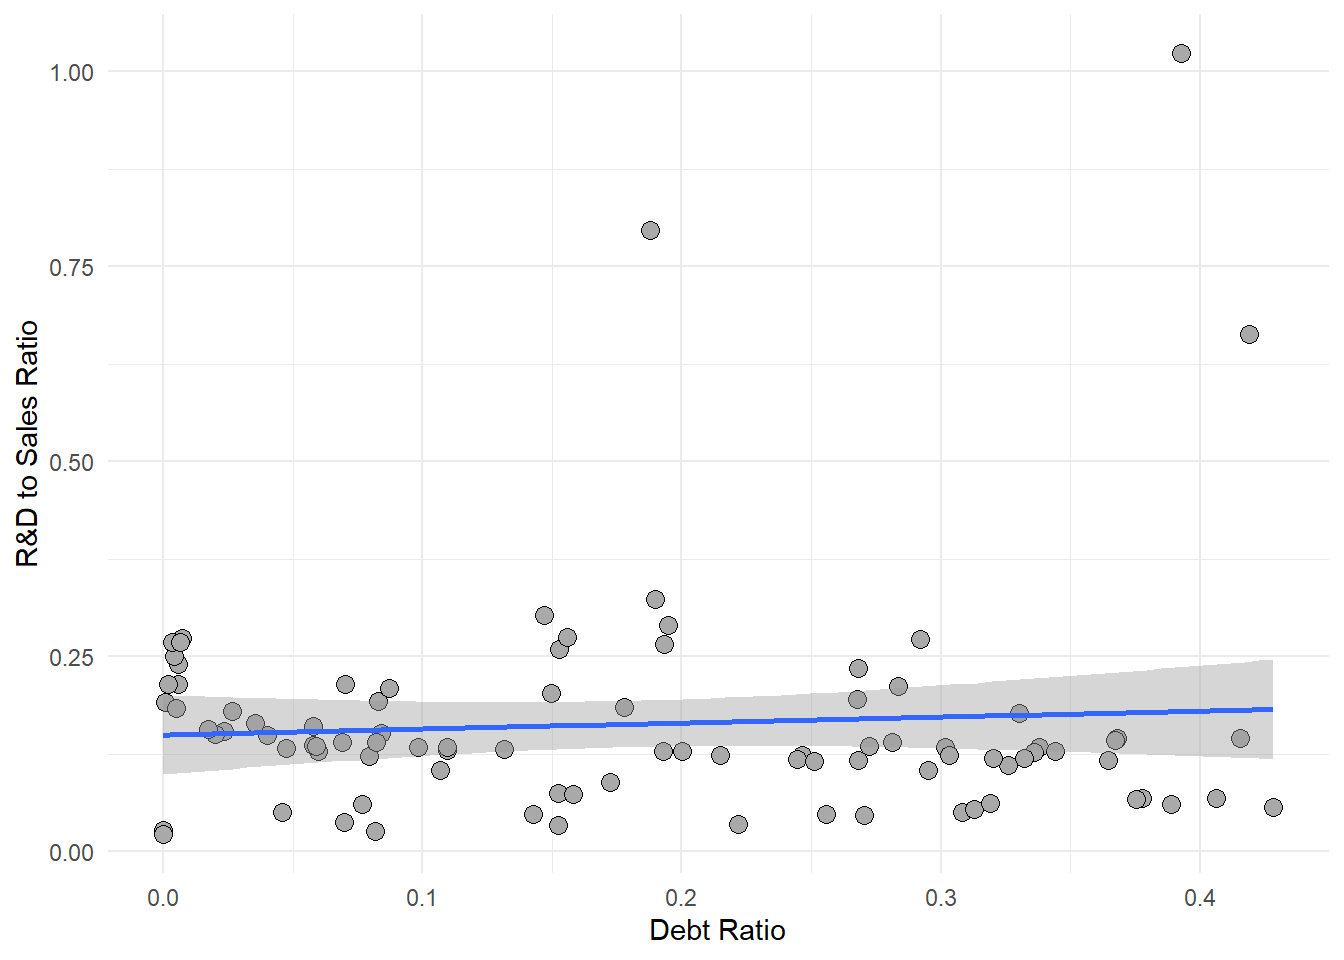
\includegraphics{Predictive-Modeling-Assignment-2_files/figure-latex/unnamed-chunk-6-1.pdf}
Our linear model looks to possibly be not normal because there a lot of
points on the top end that do not follow the normal curve, along with it
not following homoskedasticity / not equal variance because in our
residuals vs fitted plot the points begin spreading out like \textless{}
when they should be equidistant and not have a pattern. Looking at our
Cook's distance there is no point's that go past the 0.5 threshold so
there seems to be no influential points.

\begin{enumerate}
\def\labelenumi{(\alph{enumi})}
\setcounter{enumi}{4}
\tightlist
\item
  Use the * and : symbols to fit linear regression models with
  interaction effects. Do any interactions appear to be statistically
  significant?
\end{enumerate}

\begin{Shaded}
\begin{Highlighting}[]
\NormalTok{auto\_lm\_int }\OtherTok{=} \FunctionTok{lm}\NormalTok{(mpg}\SpecialCharTok{\textasciitilde{}}\NormalTok{.}\SpecialCharTok{*}\NormalTok{. , }\AttributeTok{data =}\NormalTok{ auto\_no\_name)}
\FunctionTok{summary}\NormalTok{(auto\_lm\_int)}
\end{Highlighting}
\end{Shaded}

\begin{verbatim}
## 
## Call:
## lm(formula = mpg ~ . * ., data = auto_no_name)
## 
## Residuals:
##     Min      1Q  Median      3Q     Max 
## -7.6303 -1.4481  0.0596  1.2739 11.1386 
## 
## Coefficients:
##                             Estimate Std. Error t value Pr(>|t|)   
## (Intercept)                3.548e+01  5.314e+01   0.668  0.50475   
## cylinders                  6.989e+00  8.248e+00   0.847  0.39738   
## displacement              -4.785e-01  1.894e-01  -2.527  0.01192 * 
## horsepower                 5.034e-01  3.470e-01   1.451  0.14769   
## weight                     4.133e-03  1.759e-02   0.235  0.81442   
## acceleration              -5.859e+00  2.174e+00  -2.696  0.00735 **
## year                       6.974e-01  6.097e-01   1.144  0.25340   
## origin                    -2.090e+01  7.097e+00  -2.944  0.00345 **
## cylinders:displacement    -3.383e-03  6.455e-03  -0.524  0.60051   
## cylinders:horsepower       1.161e-02  2.420e-02   0.480  0.63157   
## cylinders:weight           3.575e-04  8.955e-04   0.399  0.69000   
## cylinders:acceleration     2.779e-01  1.664e-01   1.670  0.09584 . 
## cylinders:year            -1.741e-01  9.714e-02  -1.793  0.07389 . 
## cylinders:origin           4.022e-01  4.926e-01   0.816  0.41482   
## displacement:horsepower   -8.491e-05  2.885e-04  -0.294  0.76867   
## displacement:weight        2.472e-05  1.470e-05   1.682  0.09342 . 
## displacement:acceleration -3.479e-03  3.342e-03  -1.041  0.29853   
## displacement:year          5.934e-03  2.391e-03   2.482  0.01352 * 
## displacement:origin        2.398e-02  1.947e-02   1.232  0.21875   
## horsepower:weight         -1.968e-05  2.924e-05  -0.673  0.50124   
## horsepower:acceleration   -7.213e-03  3.719e-03  -1.939  0.05325 . 
## horsepower:year           -5.838e-03  3.938e-03  -1.482  0.13916   
## horsepower:origin          2.233e-03  2.930e-02   0.076  0.93931   
## weight:acceleration        2.346e-04  2.289e-04   1.025  0.30596   
## weight:year               -2.245e-04  2.127e-04  -1.056  0.29182   
## weight:origin             -5.789e-04  1.591e-03  -0.364  0.71623   
## acceleration:year          5.562e-02  2.558e-02   2.174  0.03033 * 
## acceleration:origin        4.583e-01  1.567e-01   2.926  0.00365 **
## year:origin                1.393e-01  7.399e-02   1.882  0.06062 . 
## ---
## Signif. codes:  0 '***' 0.001 '**' 0.01 '*' 0.05 '.' 0.1 ' ' 1
## 
## Residual standard error: 2.695 on 363 degrees of freedom
##   (5 observations deleted due to missingness)
## Multiple R-squared:  0.8893, Adjusted R-squared:  0.8808 
## F-statistic: 104.2 on 28 and 363 DF,  p-value: < 2.2e-16
\end{verbatim}

Using an alpha level of 0.05, the following interactions are
significant: displacement:year,acceleration:year, and
acceleration:origin.

\begin{enumerate}
\def\labelenumi{(\alph{enumi})}
\setcounter{enumi}{5}
\tightlist
\item
  Try a few different transformations of the variables, such as log(X),
  √ X, X2. Comment on your findings
\end{enumerate}

\begin{Shaded}
\begin{Highlighting}[]
\NormalTok{auto\_lm\_trans }\OtherTok{=} \FunctionTok{lm}\NormalTok{(mpg}\SpecialCharTok{\textasciitilde{}}\FunctionTok{log}\NormalTok{(horsepower)}\SpecialCharTok{+}\NormalTok{horsepower, }\AttributeTok{data=}\NormalTok{auto\_no\_name)}
\FunctionTok{summary}\NormalTok{(auto\_lm\_trans)}
\end{Highlighting}
\end{Shaded}

\begin{verbatim}
## 
## Call:
## lm(formula = mpg ~ log(horsepower) + horsepower, data = auto_no_name)
## 
## Residuals:
##      Min       1Q   Median       3Q      Max 
## -14.5118  -2.5018  -0.2533   2.4446  15.3102 
## 
## Coefficients:
##                  Estimate Std. Error t value Pr(>|t|)    
## (Intercept)     156.04057   12.08267  12.914  < 2e-16 ***
## log(horsepower) -31.59815    3.28363  -9.623  < 2e-16 ***
## horsepower        0.11846    0.02929   4.044 6.34e-05 ***
## ---
## Signif. codes:  0 '***' 0.001 '**' 0.01 '*' 0.05 '.' 0.1 ' ' 1
## 
## Residual standard error: 4.415 on 389 degrees of freedom
##   (5 observations deleted due to missingness)
## Multiple R-squared:  0.6817, Adjusted R-squared:  0.6801 
## F-statistic: 416.6 on 2 and 389 DF,  p-value: < 2.2e-16
\end{verbatim}

\begin{Shaded}
\begin{Highlighting}[]
\FunctionTok{par}\NormalTok{(}\AttributeTok{mfrow=}\FunctionTok{c}\NormalTok{(}\DecValTok{2}\NormalTok{,}\DecValTok{2}\NormalTok{))}
\FunctionTok{plot}\NormalTok{(auto\_lm\_trans)}
\end{Highlighting}
\end{Shaded}

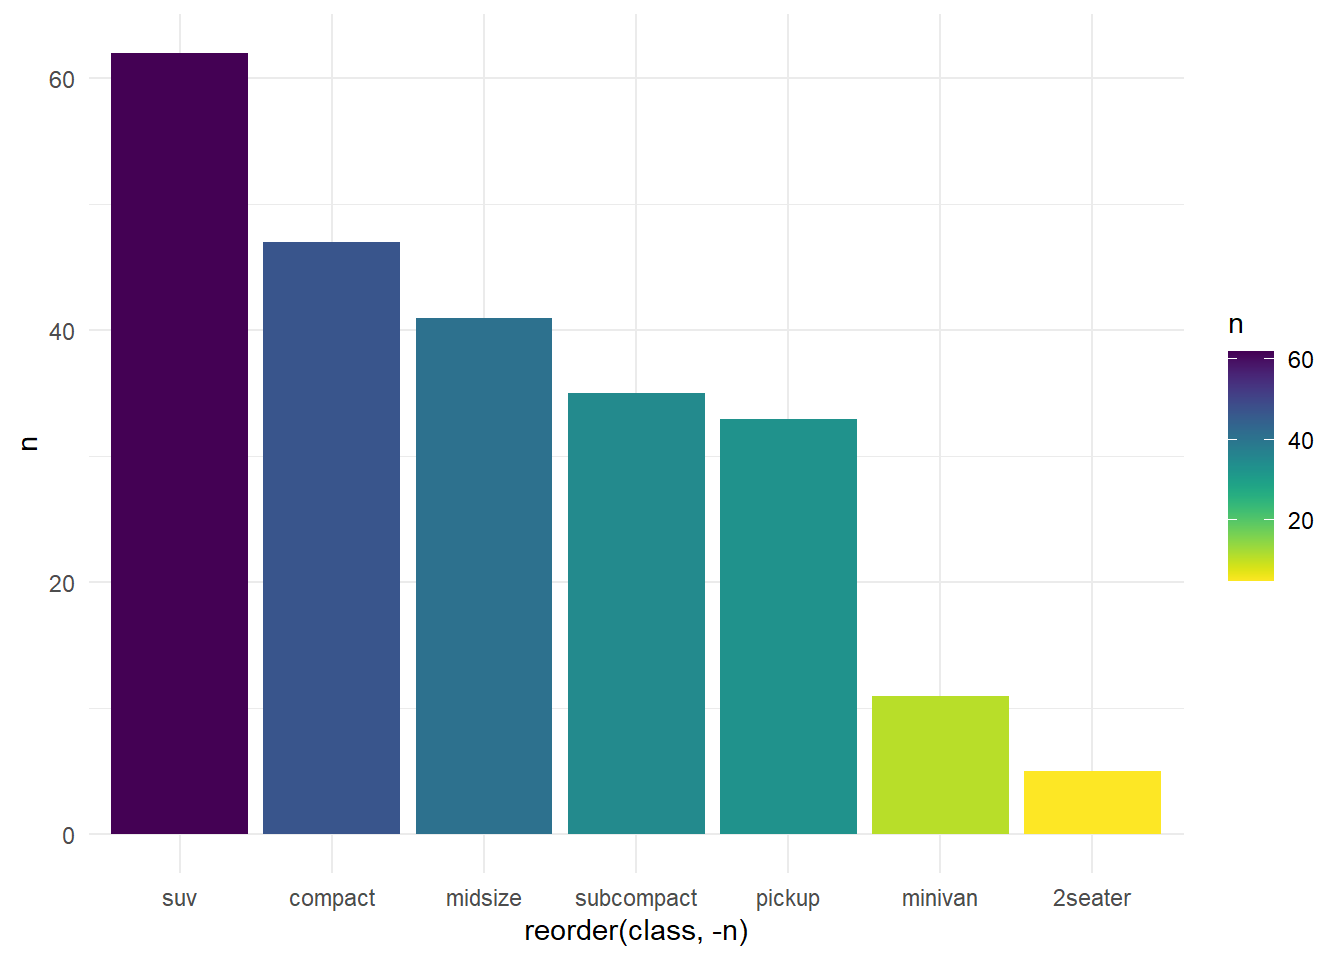
\includegraphics{Predictive-Modeling-Assignment-2_files/figure-latex/unnamed-chunk-9-1.pdf}
Previously, horsepower was not significant when including all variables
of the model but now it became significant with the transformation. It
also seems to follow normality and equal variance more than the entire
model.

\hypertarget{section}{%
\subsection{10.}\label{section}}

\begin{Shaded}
\begin{Highlighting}[]
\NormalTok{carsets }\OtherTok{\textless{}{-}} \FunctionTok{read.csv}\NormalTok{(}\StringTok{"\textasciitilde{}/R{-}Studio/Predictive Modeling/ALL CSV FILES {-} 2nd Edition/Carseats.csv"}\NormalTok{)}
\end{Highlighting}
\end{Shaded}

\begin{enumerate}
\def\labelenumi{(\alph{enumi})}
\tightlist
\item
  Fit a multiple regression model to predict Sales using Price, Urban,
  and US.
\end{enumerate}

\begin{Shaded}
\begin{Highlighting}[]
\NormalTok{carseats\_lm }\OtherTok{=} \FunctionTok{lm}\NormalTok{(Sales }\SpecialCharTok{\textasciitilde{}}\NormalTok{ Price }\SpecialCharTok{+}\NormalTok{ Urban }\SpecialCharTok{+}\NormalTok{ US, }\AttributeTok{data =}\NormalTok{ carsets)}
\FunctionTok{summary}\NormalTok{(carseats\_lm)}
\end{Highlighting}
\end{Shaded}

\begin{verbatim}
## 
## Call:
## lm(formula = Sales ~ Price + Urban + US, data = carsets)
## 
## Residuals:
##     Min      1Q  Median      3Q     Max 
## -6.9206 -1.6220 -0.0564  1.5786  7.0581 
## 
## Coefficients:
##              Estimate Std. Error t value Pr(>|t|)    
## (Intercept) 13.043469   0.651012  20.036  < 2e-16 ***
## Price       -0.054459   0.005242 -10.389  < 2e-16 ***
## UrbanYes    -0.021916   0.271650  -0.081    0.936    
## USYes        1.200573   0.259042   4.635 4.86e-06 ***
## ---
## Signif. codes:  0 '***' 0.001 '**' 0.01 '*' 0.05 '.' 0.1 ' ' 1
## 
## Residual standard error: 2.472 on 396 degrees of freedom
## Multiple R-squared:  0.2393, Adjusted R-squared:  0.2335 
## F-statistic: 41.52 on 3 and 396 DF,  p-value: < 2.2e-16
\end{verbatim}

\begin{enumerate}
\def\labelenumi{(\alph{enumi})}
\setcounter{enumi}{1}
\item
  Provide an interpretation of each coefficient in the model. Be
  careful---some of the variables in the model are qualitative! Price:
  With all other variables held constant, a one unit increase in price
  is a loss of 0.054459 sales. Urban: With all other variables held
  constant, if a store is in an urban area, then there is a loss of
  0.021916 sales. US: With all other variables held constant, if a store
  is in the US, then there is a 1.200573 increase in sales.
\item
  Write out the model in equation form, being careful to handle the
  qualitative variables properly. 3.7 Exercises 125
\end{enumerate}

Sales = 13.043469 - 0.054459 * (Price) - 0.021916 * (Urban) + 1.200573 *
(US) Urban and US can be 0 or 1 to nullify their part of the equation.

\begin{enumerate}
\def\labelenumi{(\alph{enumi})}
\setcounter{enumi}{3}
\tightlist
\item
  For which of the predictors can you reject the null hypothesis H0 : βj
  = 0?
\end{enumerate}

Price and US, assuming 0.05

\begin{enumerate}
\def\labelenumi{(\alph{enumi})}
\setcounter{enumi}{4}
\tightlist
\item
  On the basis of your response to the previous question, fit a smaller
  model that only uses the predictors for which there is evidence of
  association with the outcome.
\end{enumerate}

\begin{Shaded}
\begin{Highlighting}[]
\NormalTok{carseat\_e }\OtherTok{=} \FunctionTok{lm}\NormalTok{(Sales }\SpecialCharTok{\textasciitilde{}}\NormalTok{ Price }\SpecialCharTok{+}\NormalTok{ US, }\AttributeTok{data =}\NormalTok{ carsets)}
\FunctionTok{summary}\NormalTok{(carseat\_e)}
\end{Highlighting}
\end{Shaded}

\begin{verbatim}
## 
## Call:
## lm(formula = Sales ~ Price + US, data = carsets)
## 
## Residuals:
##     Min      1Q  Median      3Q     Max 
## -6.9269 -1.6286 -0.0574  1.5766  7.0515 
## 
## Coefficients:
##             Estimate Std. Error t value Pr(>|t|)    
## (Intercept) 13.03079    0.63098  20.652  < 2e-16 ***
## Price       -0.05448    0.00523 -10.416  < 2e-16 ***
## USYes        1.19964    0.25846   4.641 4.71e-06 ***
## ---
## Signif. codes:  0 '***' 0.001 '**' 0.01 '*' 0.05 '.' 0.1 ' ' 1
## 
## Residual standard error: 2.469 on 397 degrees of freedom
## Multiple R-squared:  0.2393, Adjusted R-squared:  0.2354 
## F-statistic: 62.43 on 2 and 397 DF,  p-value: < 2.2e-16
\end{verbatim}

\begin{enumerate}
\def\labelenumi{(\alph{enumi})}
\setcounter{enumi}{5}
\tightlist
\item
  How well do the models in (a) and (e) fit the data?
\end{enumerate}

Using Adjusted R-squared, Model A is 0.2335 and Model E is 0.2354. This
means that both models can explain \textasciitilde23\% of variance but
Model E has a better F statistic at 62.43 which is \textasciitilde20
higher than Model A.

\begin{enumerate}
\def\labelenumi{(\alph{enumi})}
\setcounter{enumi}{6}
\tightlist
\item
  Using the model from (e), obtain 95 \% confidence intervals for the
  coefficient(s).
\end{enumerate}

\begin{Shaded}
\begin{Highlighting}[]
\FunctionTok{confint}\NormalTok{(carseat\_e)}
\end{Highlighting}
\end{Shaded}

\begin{verbatim}
##                   2.5 %      97.5 %
## (Intercept) 11.79032020 14.27126531
## Price       -0.06475984 -0.04419543
## USYes        0.69151957  1.70776632
\end{verbatim}

There is a 95\% chance that the values of price fall between
(-0.06475984, -0.04419543) and ( 0.69151957, 1.70776632) for US and a
5\% chance it does not.

\begin{enumerate}
\def\labelenumi{(\alph{enumi})}
\setcounter{enumi}{7}
\tightlist
\item
  Is there evidence of outliers or high leverage observations in the
  model from (e)?
\end{enumerate}

\begin{Shaded}
\begin{Highlighting}[]
\FunctionTok{par}\NormalTok{(}\AttributeTok{mfrow=}\FunctionTok{c}\NormalTok{(}\DecValTok{2}\NormalTok{,}\DecValTok{2}\NormalTok{))}
\FunctionTok{plot}\NormalTok{(carseat\_e)}
\end{Highlighting}
\end{Shaded}

\includegraphics{Predictive-Modeling-Assignment-2_files/figure-latex/unnamed-chunk-14-1.pdf}
Looks like there are no high leverage observations in the Residuals vs
Leverage plot.

\hypertarget{this-problem-involves-simple-linear-regression-without-an-intercept.}{%
\subsection{12.This problem involves simple linear regression without an
intercept.}\label{this-problem-involves-simple-linear-regression-without-an-intercept.}}

\begin{enumerate}
\def\labelenumi{(\alph{enumi})}
\tightlist
\item
  Recall that the coefficient estimate βˆ for the linear regression of Y
  onto X without an intercept is given by (3.38). Under what
  circumstance is the coefficient estimate for the regression of X onto
  Y the same as the coefficient estimate for the regression of Y onto X?
\end{enumerate}

When the coefficient is 1 they should be the same?

\begin{enumerate}
\def\labelenumi{(\alph{enumi})}
\setcounter{enumi}{1}
\tightlist
\item
  Generate an example in R with n = 100 observations in which the
  coefficient estimate for the regression of X onto Y is different from
  the coefficient estimate for the regression of Y onto X.
\end{enumerate}

\begin{Shaded}
\begin{Highlighting}[]
\NormalTok{x }\OtherTok{=} \FunctionTok{rnorm}\NormalTok{(}\DecValTok{100}\NormalTok{)}
\NormalTok{y }\OtherTok{=} \FloatTok{0.42}\SpecialCharTok{*}\NormalTok{x }\SpecialCharTok{+} \FunctionTok{rnorm}\NormalTok{(}\DecValTok{100}\NormalTok{)}
\NormalTok{q12\_a }\OtherTok{=} \FunctionTok{lm}\NormalTok{(y}\SpecialCharTok{\textasciitilde{}}\NormalTok{x)}
\NormalTok{q12\_b }\OtherTok{=} \FunctionTok{lm}\NormalTok{(x}\SpecialCharTok{\textasciitilde{}}\NormalTok{y)}
\FunctionTok{summary}\NormalTok{(q12\_a)}
\end{Highlighting}
\end{Shaded}

\begin{verbatim}
## 
## Call:
## lm(formula = y ~ x)
## 
## Residuals:
##     Min      1Q  Median      3Q     Max 
## -2.8719 -0.8055 -0.1087  0.7455  2.4459 
## 
## Coefficients:
##             Estimate Std. Error t value Pr(>|t|)    
## (Intercept) -0.01557    0.11029  -0.141    0.888    
## x            0.55447    0.11449   4.843 4.78e-06 ***
## ---
## Signif. codes:  0 '***' 0.001 '**' 0.01 '*' 0.05 '.' 0.1 ' ' 1
## 
## Residual standard error: 1.098 on 98 degrees of freedom
## Multiple R-squared:  0.1931, Adjusted R-squared:  0.1849 
## F-statistic: 23.45 on 1 and 98 DF,  p-value: 4.783e-06
\end{verbatim}

\begin{Shaded}
\begin{Highlighting}[]
\FunctionTok{summary}\NormalTok{(q12\_b)}
\end{Highlighting}
\end{Shaded}

\begin{verbatim}
## 
## Call:
## lm(formula = x ~ y)
## 
## Residuals:
##     Min      1Q  Median      3Q     Max 
## -2.2703 -0.5980  0.1168  0.6107  1.7787 
## 
## Coefficients:
##             Estimate Std. Error t value Pr(>|t|)    
## (Intercept)  0.08011    0.08704   0.920     0.36    
## y            0.34827    0.07191   4.843 4.78e-06 ***
## ---
## Signif. codes:  0 '***' 0.001 '**' 0.01 '*' 0.05 '.' 0.1 ' ' 1
## 
## Residual standard error: 0.8701 on 98 degrees of freedom
## Multiple R-squared:  0.1931, Adjusted R-squared:  0.1849 
## F-statistic: 23.45 on 1 and 98 DF,  p-value: 4.783e-06
\end{verbatim}

\begin{Shaded}
\begin{Highlighting}[]
\FunctionTok{coefficients}\NormalTok{(q12\_a)}
\end{Highlighting}
\end{Shaded}

\begin{verbatim}
## (Intercept)           x 
## -0.01557122  0.55446902
\end{verbatim}

\begin{Shaded}
\begin{Highlighting}[]
\FunctionTok{coefficients}\NormalTok{(q12\_b)}
\end{Highlighting}
\end{Shaded}

\begin{verbatim}
## (Intercept)           y 
##  0.08011264  0.34827428
\end{verbatim}

They are different

\begin{enumerate}
\def\labelenumi{(\alph{enumi})}
\setcounter{enumi}{2}
\tightlist
\item
  Generate an example in R with n = 100 observations in which the
  coefficient estimate for the regression of X onto Y is the same as the
  coefficient estimate for the regression of Y onto X
\end{enumerate}

\begin{Shaded}
\begin{Highlighting}[]
\NormalTok{x }\OtherTok{=} \FunctionTok{rnorm}\NormalTok{(}\DecValTok{100}\NormalTok{)}
\NormalTok{y }\OtherTok{=}\NormalTok{ x }
\NormalTok{q12\_c }\OtherTok{=} \FunctionTok{lm}\NormalTok{(y}\SpecialCharTok{\textasciitilde{}}\NormalTok{x)}
\NormalTok{q12\_d }\OtherTok{=} \FunctionTok{lm}\NormalTok{(x}\SpecialCharTok{\textasciitilde{}}\NormalTok{y)}
\FunctionTok{summary}\NormalTok{(q12\_c)}
\end{Highlighting}
\end{Shaded}

\begin{verbatim}
## Warning in summary.lm(q12_c): essentially perfect fit: summary may be
## unreliable
\end{verbatim}

\begin{verbatim}
## 
## Call:
## lm(formula = y ~ x)
## 
## Residuals:
##        Min         1Q     Median         3Q        Max 
## -1.466e-15  2.210e-18  1.303e-17  3.018e-17  1.554e-16 
## 
## Coefficients:
##              Estimate Std. Error   t value Pr(>|t|)    
## (Intercept) 2.220e-17  1.581e-17 1.404e+00    0.163    
## x           1.000e+00  1.900e-17 5.264e+16   <2e-16 ***
## ---
## Signif. codes:  0 '***' 0.001 '**' 0.01 '*' 0.05 '.' 0.1 ' ' 1
## 
## Residual standard error: 1.56e-16 on 98 degrees of freedom
## Multiple R-squared:      1,  Adjusted R-squared:      1 
## F-statistic: 2.771e+33 on 1 and 98 DF,  p-value: < 2.2e-16
\end{verbatim}

\begin{Shaded}
\begin{Highlighting}[]
\FunctionTok{summary}\NormalTok{(q12\_d)}
\end{Highlighting}
\end{Shaded}

\begin{verbatim}
## Warning in summary.lm(q12_d): essentially perfect fit: summary may be
## unreliable
\end{verbatim}

\begin{verbatim}
## 
## Call:
## lm(formula = x ~ y)
## 
## Residuals:
##        Min         1Q     Median         3Q        Max 
## -1.466e-15  2.210e-18  1.303e-17  3.018e-17  1.554e-16 
## 
## Coefficients:
##              Estimate Std. Error   t value Pr(>|t|)    
## (Intercept) 2.220e-17  1.581e-17 1.404e+00    0.163    
## y           1.000e+00  1.900e-17 5.264e+16   <2e-16 ***
## ---
## Signif. codes:  0 '***' 0.001 '**' 0.01 '*' 0.05 '.' 0.1 ' ' 1
## 
## Residual standard error: 1.56e-16 on 98 degrees of freedom
## Multiple R-squared:      1,  Adjusted R-squared:      1 
## F-statistic: 2.771e+33 on 1 and 98 DF,  p-value: < 2.2e-16
\end{verbatim}

\begin{Shaded}
\begin{Highlighting}[]
\FunctionTok{coefficients}\NormalTok{(q12\_c)}
\end{Highlighting}
\end{Shaded}

\begin{verbatim}
##  (Intercept)            x 
## 2.220446e-17 1.000000e+00
\end{verbatim}

\begin{Shaded}
\begin{Highlighting}[]
\FunctionTok{coefficients}\NormalTok{(q12\_d)}
\end{Highlighting}
\end{Shaded}

\begin{verbatim}
##  (Intercept)            y 
## 2.220446e-17 1.000000e+00
\end{verbatim}

Now they are the same / perfect fit.

\end{document}
